\documentclass[twocolumn]{IEEEtran}
\usepackage{graphicx}
\usepackage[utf8x]{inputenc}
\usepackage{times}
\usepackage{amssymb,amsfonts}
\usepackage[tbtags]{amsmath}
\usepackage{cite}
\usepackage{pict2e}
\usepackage{float}
\usepackage{lscape}
\usepackage[all]{xy}
\usepackage{graphics,graphicx,color,colortbl}
\usepackage{times}
\usepackage{subfigure}
\usepackage{wrapfig}
\usepackage{multicol}
\usepackage{cite}
\usepackage{url}
\usepackage[tbtags]{amsmath}
\usepackage{amsmath,amssymb,amsfonts,amsbsy}
\usepackage{listings}
\usepackage{bm}
%\usepackage{algorithm}
%\usepackage{algorithmic}
\usepackage[centerlast, small]{caption}
\usepackage[colorlinks=true, citecolor=blue, linkcolor=blue, urlcolor=blue, breaklinks=true]{hyperref}
\hyphenation{ele-men-tos he-rra-mi-en-ta cons-tru-yen trans-fe-ren-ci-a pro-pu-es-tas si-mu-lar vi-sua-li-za-cion}

\begin{document}
\title{Analisis de desempeño: Communication on Chip}
\author{David Ricardo Martínez Hernández \textbf{Código:} $261931$\\
	Sergio Ándres Zapata Palomino \textbf{Código:} $261261$}
\maketitle
\markboth{Universidad Nacional de Colombia}{}
\floatname{algorithm}{Algoritmo}

\begin{abstract}
 En este informe se analizan las principales características de un bus simple, y como éste es descrito mediante código en System C. Mediante este código se diseñan nuevos sistemas de buses simples observando así las relaciones de precedencia entre los master del bus. También se observan criterios en las métricas de desempeño, como la latencia, el throughput y el nivel de utilización. Finalmente se describen diferentes políticas de arbitraje para así establecer mediante métricas de desempeño cual es mejor. A partir de los resultados obtenidos se plantean las coclusiones.
\end{abstract}

\begin{keywords}
 Bus, Master, Slave, SystemC.
\end{keywords}

\section{Introducción}
\noindent
Los sistemas constituidos sobre un solo chip  deben poseer redes que sean capaces de comunicar los generadores de información maestros con los receptores o esclavos.\\
Estas redes deben tener capacidad de interactuar dentro el sistema minimizando las pérdidas en energía y velocidad en la transacción de los paquetes que viajan a través de ellos, existen muchas implementaciones como por mencionar \textbf{Mbus}, \textbf{Simple Bus}, \textbf{NoC}, cada una de ellas con diferentes formas de abordar el problema.\\
En este laboratorio se modificara un sistema Simple Bus, teniendo la posibilidad de implementar el modelo de comunicación, y definir la política de arbitraje a \textbf{TMDA}, luego comparar el desempeño con una política de arbitraje de prioridad fija.\\
Luego cuantificar el desempeño por las métricas de latencia, Thoughtput y nivel de utilización.
\begin{itemize}
 \item \textbf{Nivel de Utilización:} que debe mostrar cuanto de la estructura de comunicación se está utilizando.
 \item \textbf{Latencia:} es una medida del tiempo que el sistema tarda en producir resultados.
 \item \textbf{Throughput:} es la cantidad de trabajos o tareas completadas por el sistema por unidad de tiempo.
\end{itemize}

\section{Marco Teórico}
\subsection{Bus}
\noindent
Es un sistema digital que transfiere datos entre los componentes de una computadora o entre computadoras. Está formado por cables o pistas en un circuito impreso, dispositivos como resistores y condensadores además de circuitos integrados\cite{page1}. Existen diferentes tipos de buses, uno de ellos es el bus simple el cual se caracteriza por no tener un sistema de \textit{pipelining} , ni de transacción dividida ni tampoco posee estados de espera por parte de los Master. Un bus permite la comunicación entre un maestro y un esclavo. La forma en la que se realiza esta comunicación se puede dividir en interfaces:
\begin{itemize}
 \item \textbf{Blocking:} La información se transmite en ráfagas.
 \item \textbf{Non-blocking}: La información se transmite un dato a la vez de acuerdo al ciclo de reloj.
 \item \textbf{Direct:} Su principal característica es que tiene un acceso directo al bus y al esclavo.
\end{itemize}

\subsection{Políticas de Arbitraje.}
\subsubsection{Round Robin}
\noindent
Es un método para seleccionar todos los elementos en un grupo de manera equitativa y en un orden racional, normalmente comenzando por el primer elemento de la lista hasta llegar al último y empezando de nuevo desde el primer elemento.\\
Una forma sencilla de entender el round robin es imaginar una secuencia para "tomar turnos" (ver Fig~\ref{fig7}).
\begin{figure}
  \centering
 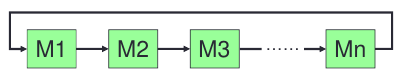
\includegraphics[scale=0.5]{fig7.png}
 \caption{Diagrama Round Robin}
 \label{fig7}
\end{figure}

\subsubsection{TDMA (Time Division Multiple Access)}
\noindent
Es un método que permite a varios elementos compartir el mismo canal dividiendo la prioridad en intervalos de tiempo (Ver Fig~\ref{fig8})
\begin{figure}
\centering
 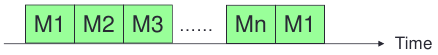
\includegraphics[scale=0.5]{fig8.png}
  \caption{Diagrama TDMA}
 \label{fig8}
\end{figure}

\subsubsection{Fixed priority}
\noindent
A cada master se le asigna un número de prioridad, entre menor sea el número mayor sera la prioridad del master. Este número siempre sera respetado durante todo el proceso (ver Fig.~\ref{fig9}):
\begin{figure}
\centering
 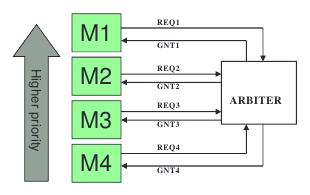
\includegraphics[scale=0.5]{fig9.png}
  \caption{Diagrama Fixed priority}
 \label{fig9}
\end{figure}

\section{Análisis de Resultados}
\noindent
Para poder realizar esta práctica es necesario ejecutar el ejemplo ``simple\_bus'', el cual se encuentra en la carpeta \textbf{\textit{systemc-2.3.0/examples/sysc/simple\_bus}}, se utilizó el Makefile desarrollado durante el semestre para la correcta ejecución de SystemC.

\subsection{Compilación y ejecución del ejemplo simple\_bus de SystemC-2.3.0.}
\noindent
Al ejecutar el ejemplo sin ninguna modificación, ejecutando en la consola \textit{make all}, se obtuvo el siguiente resultado (Fig.~\ref{fig1})
\begin{figure}[H]
  \centering
    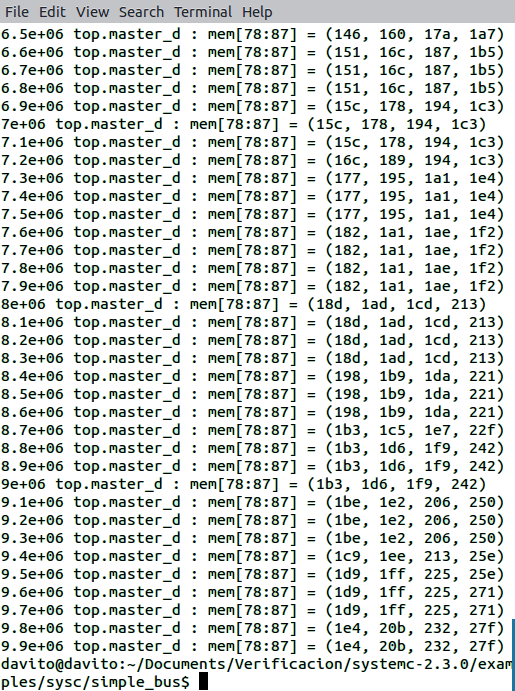
\includegraphics[scale=0.48]{fig1.png}
  \caption{Salida de la simulación del ejemplo sin ninguna modificación.}
 \label{fig1}
\end{figure}
\noindent
Como se puede observar en la Fig.~\ref{fig1} el master direct tiene siempre ocupado el Bus y no se lo sede a ningún otro master por la prioridad que tiene, su prioridad es siempre respondida sin importar quien tenga ocupado el Bus.\\
Pero para poder observar quien tenia ocupado el bus y como se encontraban las políticas de arbitraje fue necesario modificar las las siguientes lineas con el siguiente código:
\lstset{numbers=left, numberstyle=\footnotesize , stepnumber=1, numbersep=1pt}
\begin{lstlisting}[firstnumber=78, caption=Código modificado., label=code1]
 bus = new simple_bus("bus",true);
 arbiter = new simple_bus_arbiter     ("arbiter", false);
\end{lstlisting}
\noindent
Se simulo nuevamente con esas instrucciones habilitadas y se obtuvo o siguiente:
\begin{figure}[H]
  \centering
    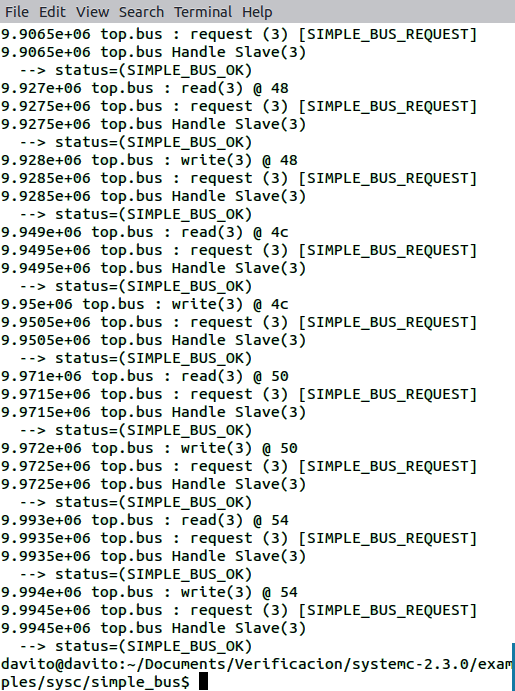
\includegraphics[scale=0.48]{fig2.png}
  \caption{Salida de la simulación del ejemplo con al modificación del Listing~\ref{code1}.}
 \label{fig2}
\end{figure}

\subsection{Sistema de bus simple con dos Master Blocking, dos Master not Blocking y un Slave slow memory.}
\noindent
Para generar este sistema es necesario modificar el código de la libreria \textit{\textbf{simple\_bus\_text.h}}, y debe quedar de la siguiente manera:
\lstset{numbers=left, numberstyle=\footnotesize , stepnumber=1, numbersep=1pt}
\begin{lstlisting}[firstnumber=41, caption=Código modificado en la definición de las librerías., label=code2]
#include "simple_bus_master_blocking.h"
#include               "simple_bus_master_non_blocking.h"
#include "simple_bus_slow_mem.h"
#include "simple_bus.h"
#include "simple_bus_arbiter.h"
#include "simple_bus_test.h"
\end{lstlisting}
\lstset{numbers=left, numberstyle=\footnotesize , stepnumber=1, numbersep=1pt}
\begin{lstlisting}[firstnumber=50, caption=Código modificado para la definición de las instancias., label=code3]
SC_MODULE(simple_bus_test)
{
 // channels
 sc_clock C1;

 // module instances
 simple_bus_master_blocking     *master_b;
 simple_bus_master_non_blocking     *master_nb;
 simple_bus_master_blocking     *master_b_2;
 simple_bus_master_non_blocking    *master_nb_2;
 simple_bus_slow_mem 6*mem_slow;
 simple_bus *bus;
 simple_bus_arbiter *arbiter;
\end{lstlisting}
\noindent
En el Listing~\ref{code3} se puede observar que ya se han declarado los masters solicitados en la entre las líneas $58$ y $59$.
\lstset{numbers=left, numberstyle=\footnotesize , stepnumber=1, numbersep=1pt}
\begin{lstlisting}[firstnumber=66, caption=Código modificado para la declaración del constructor., label=code4]
// constructor
SC_CTOR(simple_bus_test)
 : C1("C1")
{
 // create instances
 master_b = new        simple_bus_master_blocking    ("master_b", 4, 0x4c, false, 10000);
 master_nb = new       simple_bus_master_non_blocking      ("master_nb", 3, 0x38, false, 10000);
 master_b_2 = new        simple_bus_master_blocking        ("master_b_2", 1, 0x24, false, 10000);
 master_nb_2 = new        simple_bus_master_non_blocking        ("master_nb_2", 2, 0x10, false, 10000);
 mem_slow = new         simple_bus_slow_mem         ("mem_slow", 0x00, 0xff, 1);
 bus = new simple_bus("bus",true);            // verbose output
 arbiter = new              simple_bus_arbiter("arbiter", false);
\end{lstlisting}
\lstset{numbers=left, numberstyle=\footnotesize , stepnumber=1, numbersep=1pt}
\begin{lstlisting}[firstnumber=83, caption=Código modificado para la declaración del clock en el constructor., label=code5]
// connect instances
bus->clock(C1);
master_b->clock(C1);
master_nb->clock(C1);
mem_slow->clock(C1);
master_b_2->clock(C1);
master_nb_2->clock(C1);
master_b->bus_port(*bus);
master_nb->bus_port(*bus);
master_b_2->bus_port(*bus);
master_nb_2->bus_port(*bus);
bus->arbiter_port(*arbiter);
bus->slave_port(*mem_slow);
\end{lstlisting}
\lstset{numbers=left, numberstyle=\footnotesize , stepnumber=1, numbersep=1pt}
\begin{lstlisting}[firstnumber=101, caption=Código modificado para la declaración del destructor., label=code6]
// destructor
~simple_bus_test()
{
 if (master_b)            {delete master_b; master_b = 0;} 
 if (master_nb)      {delete master_nb; master_nb = 0;}
 if (master_b_2)      {delete master_b; master_b_2 = 0;}
 if (master_nb_2)      {delete master_nb; master_nb_2 = 0;}
 if (mem_slow) {delete mem_slow; mem_slow = 0;}
 if (bus) {delete bus; bus = 0;}
 if (arbiter) {delete arbiter; arbiter = 0;}
\end{lstlisting}
\noindent
Al realizar los cambios anteriores se simulo nuevamente y se obtuvo el siguiente resultado (Fig.~\ref{fig3})
\begin{figure}[H]
  \centering
    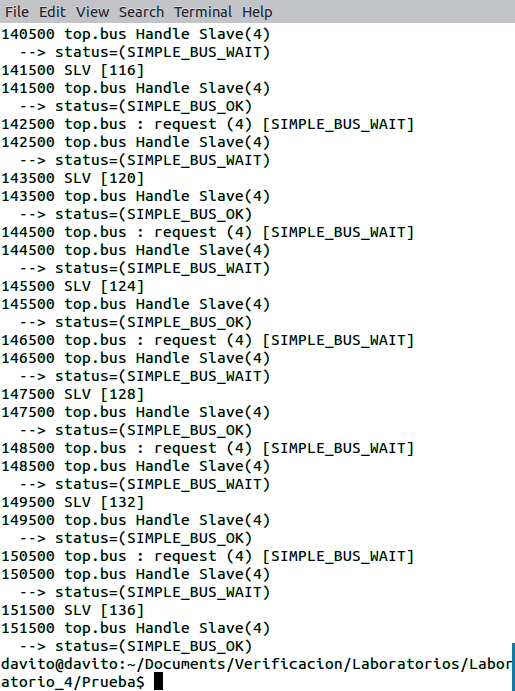
\includegraphics[scale=0.48]{fig3.png}
  \caption{Salida de la simulación al modificar el Listing~\ref{code6}.}
 \label{fig3}
\end{figure}

%\subsection{Métricas de desempeño.}
%\subsubsection{Latencia}
%noindent
%
%
%\subsubsection{Throughput}
%\noindent
%
%
%\subsubsection{Nivel de utilización}
%\noindent
%
%
\section{Pruebas extras}
\noindent
En Listing~\ref{code4} se observar creación de los cuatro masters, dos blocking y dos non-blocking, también se puede ver el grado de prioridad que tiene cada uno de estos masters la cual corresponde al primer número que aparece después de nombrarlo, entre menor sea este número, mayor será su prioridad.\\
El último número, que corresponde a $10000$ indica cada cuanto se va a hacer una request, este número se compara con el tiempo total de la simulación el cual se define en el archivo \textit{simple\_bus\_main.cpp} el cual se puede observar en el Listing~\ref{code7}
\lstset{numbers=left, numberstyle=\footnotesize , stepnumber=1, numbersep=1pt}
\begin{lstlisting}[firstnumber=36, caption=Contenido del archivo simple\_bus\_main.cpp., label=code7]
#include "systemc.h"
#include "simple_bus_test.h"

int sc_main(int, char **)
{
 simple_bus_test top("top");

 sc_start(10000, SC_NS);
 
  return 0;
}
\end{lstlisting}
\noindent
En la línea $43$ en el comando \textbf{\textit{sc\_start()}} se define el tiempo de simulación y las unidades de tiempo usadas, en este caso serán nanosegundos.\\
Al utilizar en la consola el comando \textit{./simple\_bus $\mid$ grep read} se obtuvo lo siguiente (ver Fig.~\ref{fig4}):
\begin{figure}[H]
  \centering
    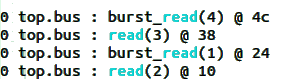
\includegraphics[scale=0.5]{fig4.png}
  \caption{Resultado al ejecutar el comando \textit{./simple\_bus $\mid$ grep read}.}
 \label{fig4}
\end{figure}
\noindent
El orden en el que aparecen estas instrucciones corresponde al orden en el que se ejecutaron las instrucciones read, se puede ver que se tomaron en el orden en que estaban inicialmente escritas en el programa sin tener en cuenta su precedencia.\\
Después de esto se ejecutó la siguiente instrucción \textit{./simple\_bus $\mid$ grep write} y se obtuvo lo siguiente en  la consola (ver Fig~\ref{fig5}).
\begin{figure}[H]
  \centering
    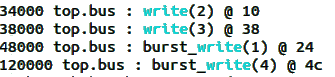
\includegraphics[scale=0.5]{fig5.png}
  \caption{Resultado al ejecutar el comando \textit{./simple\_bus $\mid$ grep write}.}
 \label{fig5}
\end{figure}
\noindent
En la imagen anterior se puede ver que el orden en el que se ejecutan las instrucciones ha cambiado, y no solo de acuerdo a su precedencia sino al tipo de master con el que se trabaja. Los primeros dos que se ejecutan son los non-blocking masters, ésto a pesar de que hay otro master con una prioridad mayor, después de estos se ejecutan los blocking masters de acuerdo a su orden de prioridad. Se puede concluir entonces que los non-blocking masters tienen prioridad sobre los blocking, incluso si su número de prioridad es mayor.\\
Posteriormente se intentó usar la misma prioridad para cada uno de los masters pero al compilarlo se obtuvo un error, por lo que se puede concluir que cada master debe tener un número de prioridad única.\\
Después de esto se volvió a habilitar el arbiter y a deshabilitar el bus para ver que resultado se obtenía. En la consola se obtuvo lo siguiente (ver Fig.~\ref{fig6}):\\
\begin{figure}[H]
  \centering
    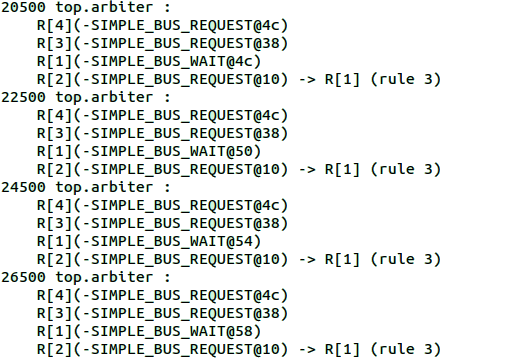
\includegraphics[scale=0.5]{fig6.png}
  \caption{Habilitación del arbiter y deshabilitación del bus.}
 \label{fig6}
\end{figure}
\noindent
En la Fig.~\ref{fig6} se puede ver una parte del resultado que se obtuvo. Aquí se puede ver como cada uno de los masters está pidiendo permiso para usar el bus. En la parte derecha se puede ver a cual de los masters se le da prioridad y de acuerdo a cual norma de arbitraje. Existen 3 normas de arbitraje, las cuales son: 
\begin{enumerate}
 \item Si la solicitud corresponde a una ``\textit{locked burst request}'' entonces a esta siempre se le dará prioridad.
 \item Si la última solicitud tiene su bandera ``\textit{lock}'' activa, y tiene una nueva solicitud  entonces se le dará prioridad a esta. 
 \item La solicitud con la mayor prioridad (menor número) es seleccionada de la cola y tomada como prioridad. 
\end{enumerate}
\noindent
Ya que no se está haciendo uso del comando ``\textit{lock}'' entonces la prioridad será regida por la norma 3. 

\section{Conclusiones}
\begin{itemize}
 \item Cuando un master non-blocking y un blocking están solicitando el bus al mismo tiempo, el master non-blocking va a tener prioridad sobre el otro, no importa el número de prioridad que tenga el master blocking. 
 \item El método de arbitraje usado por el bus simple original es el de prioridad fija, cada solicitud por parte de los master es leída en el orden de llegada, sin embargo se le da prioridad a aquel master con un número de prioridad menor. Esto siempre y cuando otro master no tenga la bandera “lock” activada o no sea un direct master, el cual tiene una prioridad directa y no tiene que esperar.
 \item En casos donde se requiera que una solicitud por parte del master para que sea atendida lo más rápido posible se podría usar la interface de bus directa, esta interface siempre va a tener la mayor prioridad, evitando así cualquier protocolo de arbitraje y la latencia que esto produce.
 \item Al umentar el número de maestros se ven afectadas las métricas porque todos los maestros comparten los mismos recursos del bus y dependiendo de las politicas de arbitraje se vera afectada la latencia.
\end{itemize}

\bibliographystyle{ieeetran}
\begin{thebibliography}{99}
\bibitem{patterson} Patterson, David \& Hennessy John
{\em "`Computer Organization And Design - The Hardware-Software Interface"'}.
Kindle Edition, Fourth Edition, 2006.

\bibitem{page1} Wikipedia. Sitio Web:\url{http://en.wikipedia.org/wiki/Bus_%28computing%29}
 . Visitado el 24 de enero de 2014.
\end{thebibliography}
\end{document}